\documentclass{report}


% General imports:
\usepackage[utf8]{inputenc}
\usepackage[T1]{fontenc}	% For using icelandic Thorn character
\usepackage{amsmath}
\usepackage{graphicx}

% Support for spanish:
\usepackage[spanish]{babel}

% Imports for images
\usepackage{caption}
\usepackage{subcaption}
\usepackage{wrapfig}

% Imports for euro symbol support
\usepackage[official]{eurosym}
\DeclareUnicodeCharacter{20AC}{\euro{}}

% Other imports:
\usepackage{indentfirst} % Indent first paragraph
\usepackage[nottoc,numbib]{tocbibind} % Add bibliography to table of contents
\usepackage{url}	% Cite URLs

% Formatting margins of the pages:
\usepackage[top=2.3cm, bottom=2.29cm, left=1.6cm, right=1.47cm]{geometry}

% Import for headers
\usepackage{fancyhdr}

% Definitions of important data
\renewcommand{\author}{David Estévez Fernández\\Enrique Fernández Rodicio\\Javier Isabel Hernández}
\renewcommand{\title}{??}
\newcommand{\department}{Máster Universitario de Robótica y Automatización\\Planificación de tareas y movimientos de robots}
\newcommand{\teacher}{Alberto Jardón Huete\\Ramón Barber Castaño}

% Define a command for comments
\usepackage{color}
\newcommand{\comment}[1]{\textbf{\color{red} #1}}

% Each chapter will have its own header
%\newcommand{\headchapter}[1]{\chapter{#1}\rhead{#1}}

% Each section will have its own header
%\newcommand{\headsection}[1]{\section{#1}}\rhead{#1}}

% Change 'Chapter' to something more logical
\renewcommand{\chaptername}{}


\begin{document}

%%%% FRONTPAGE %%%%%%%%%%%%%%%%%%%%%%%%%%%%%%%%%%%%%%%%%%%%%%%%%%%%%%%%%%%%%%%%
\newcommand{\frontpage}[4]
{
\begin{center}

\includegraphics[width=0.25\textwidth]{./images/uc3m.jpg}\\[2cm]
\textsc{\LARGE Universidad Carlos III de Madrid}\\[0.5cm]
\textsc{\Large #1}\\[3cm]


% Title
{\huge \bfseries{#2}\\[7cm]}


% Author and supervisor
\begin{minipage}{0.35\textwidth}
\begin{flushleft} \large
\emph{Autores:}\\
#3\\
\end{flushleft}
\end{minipage}
\begin{minipage}{0.4\textwidth}
\begin{flushright} \large
\emph{Profesores:}\\
#4
\end{flushright}\end{minipage}\vfill

% Bottom of the page
{\large \today}

\end{center}
%
\newpage
%
}

\frontpage{\department}{\title}{\author}{\teacher}

% Adding some header text on top of the page:
\lhead{}
\chead{}
\rhead{\title}
\pagestyle{fancy}


%%%%%%Table of contents%%%%%%%%%%%%%%%%%%%%%%%%%%%%%%%%%%%%%%%%%%%%%%%%%%%%%%%%
\tableofcontents
\newpage

%%%% Different Sections %%%%%%%%%%%%%%%%%%%%%%%%%%%%%%%%%%%%%%%%%%%%%%%%%%%%%%%
\chapter{Introducción}
\label{introduccion}

En este trabajo se explicarán dos artículos de investigación relacionados con la planificación de tareas y movimientos en robots. Más concretamente se trata de los artículos \textit{A Note on ``Solving the Find-Path Problem by Good Representation of Free Space''} y \textit{Quasi-Randomized Path Planning}.\\

Se comenzará por realizar un pequeño resumen y comentario de cada uno de ellos de forma individual, explicando los algoritmos o ideas que sus autores presentan en ellos. En caso de que sea necesario introducir alguna referencia para la comprensión del artículo asignado, también se presentará un resumen de la refencia a modo de contexto para el lector de este trabajo. Los detalles que van a ser tratados en otras secciones se omitirán de este apartado para evitar redundancias en el trabajo. Una vez presentados ambos artículos, se procederá a realizar una comparativa entre ambos algoritmos, indicando los puntos fuerte y débiles de cada uno.\\

Tras la explicación de los algoritmos presentados en los artículos principal y complementario, se prodecerá a la descripción detallada del caso de uso seleccionado para la implementación del algoritmo. Al ser muy complicada la implementación del algoritmo principal, debido a su naturaleza de crítica a ciertos aspectos concretos de otro artículo, se ha decidido implementar el algoritmo del artículo complementario. Esta sección explica el caso de uso elegido y las razones por las cuales se ha seleccionado este problema como adecuado para el algoritmo a desarrollar.\\

En la siguiente sección se tratarán de forma detallada todos los detalles de la implementación del algoritmo seleccionado, así como los detalles relativos a la simulación. Se describirá el algoritmo implementado paso a paso, haciendo incampié en los aspectos fundamentales que el autor describió en el artículo y que son indispensables para el correcto funcionamiento del algoritmo. También se tratarán las mejoras o cambios introducidos por los alumnos en el algoritmo original, así como el efecto que tiene variar los distintos parámetros del algoritmo sobre el resultado final, tanto en sus resultados y rendimiento como en el tiempo de ejecución del mismo.\\

Por último, se llevará a cabo una conclusión en la que se repasarán los elementos más significativos de este trabajo, a la vez que se reflexionará sobre los resultados obtenidos, enlazándolos y contrastándolos con los resultados presentados en los artículos originales.\\
\chapter{Artículos asignados}
\label{articulos}

En este capítulo se explicarán tanto el artículo principal con el complementario. También se incluirán explicaciones de las referencias cuando sea necesario para la correcta comprensión del artículo a tratar. Por último, se llevará a cabo una comparativa de ambos artículos.

\section{Artículo principal}
\label{articulo_principal}

\comment{Aquí se habla del artículo principal}
\section{Artículo complementario}
\label{articulo_complementario}


El articulo complementario que se ha estudiado durante la realización de este proyecto tiene por título \textsl{"Quasi-Randomized Path Planning"}, y fue escrito por M. Branicky, S. La Valle, K. Olson y L. Yang.. En el se propone un enfoque distinto a la hora de muestrear el espacio por el que se moverá el robot, pasando a distribuir los nodos de forma cuasi-aleatoria, en vez de hacerse por completo aleatoriamente.
\\

Cuando se trabaja en un espacio de configuraciones con un alto número de variables a considerar, las aproximaciones determinísticas clásicas desarrolladas para la planificación de trayectorias dejan de ser aplicables, o son demasiado costosas. Para estos casos, en la década de los 90 se comenzarom a desarrollar enfoques aleatorios. Estos métodos pasaron a ser mas usados que los determinísticos por dos motivos:
\begin{enumerate}
\item Permitían resolver un problema con una alta multidimensionalidad sin la necesidad de explorar todas las alternativas.
\item Si se ve el problema como un enemigo a vencer, a menudo se puede evitar la derrota aplicando una estrategia aleatoria, cosa que no ocurre con una determinística. 
\end{enumerate}  

Sin embargo, no es posible conseguir suna serie de datos realmente aleatorios, ya que cualquier posible implementación simplemente llevará a una secuencia determinística de números pseudoaleatorios que van a seguir una cierta función de probabilidad. De aquí se sacó la idea de desarrollar un metodo cuasi-aleatorio que permitiese solucionar el problema de la generación de trayectorias de forma más eficaz. 
\\

A la hora de generar la secuencia de muestras pseudo-aleatorias con las que va a trabajar el método aleatorio de planificación, se busca el conjunto de puntos que optimicen el valor de dos parámetros, la discrepancia y la dispersión. La discrepancia para un conjunto P formado por N muestras de d-dimensiones en $[0,1]^{d}$  viene dada por la ecuación 2.1:
\begin{equation}
D_{N}(P) = \sup_{j} |\frac{A(J)}{N}-\mu(J)|
\end{equation} 

Donde J es cualquier subconjunto rectangular perteneciente a $[0,1]^{d}$, $\mu(J)$ es su medida y A(J) es el número de puntos que pertenecen a la unión entre P y J. En cuanto a la dispersión, hace referencia a la máxima distancia a la que cada punto de un conjunto puede estar respecto al punto mas cercano perteneciente a la misma secuencia. Por lo general, los conjuntos de puntos que presentan una baja discrepancia también poseerán una baja dispersión.
\\

Se desarrollaron cuatro distintos conjuntos de muestras:
\begin{enumerate}
\item Cuadrículas: Consiste en la cuantificación uniforme de cada uno de los ejes de coordenadas.
\item Enrejado: Generalización que mantiene la estructura de una cuadrícula, pero es generado por un conjunto de bases generalmente no ortogonales que buscan obtener una baja discrepancia.
\item Método cerrado: No requiere una estructura de vecindad para las muestras, cuyo número debe ser conocido a priori.
\item Método abierto: No es necesario conocer a priori el número de muestras. Por lo general, se obtiene una discrepancia más alta entre las muestras que con el método cerrado 
\end{enumerate}

El primer grupo es un subconjunto del segundo, que a su vez es un subconjunto del tercero. Para probar los resultados que ofrece el uso del método abierto y el cerrado desarrollaron una variante del algoritmo Probabilistic Road Map (de ahora en adelante PRM), mientras que para probar los otros dos conjuntos optaron por una variación del Lazy PRM.
\\

El algoritmo PRM y sus variantes se pueden dividir en dos fases. La primera consisitiría en la generación aleatoria de nodos dentro del mapa con el que se está trabajando. Estos nodos se conectan entre sí para crear un grafo, siempre evitando generar nodos o conexiones encima de obstáculos. Una vez obtenido dicho grafo, la segunda fase consiste en encontrar el camino mas corto entre el punto inicial y el final, a través de las distintas conexiones que conforman el grafo.
\\

En cuanto al Lazy PRM, sigue la misma estructura que el PRM clásico, con una diferencia. Durante la primera fase, al generar el grafo, no se tienen en cuenta los obstáculos al distribuir los nodos y crear las conexiones entre ellos. Después, se usa un algoritmo para encontrar el camino a través del grafo (en este caso se ha usado el A*) y se genera una trayectoria. Por último, se comprueba si alguno de los tramos del camino colisiona con un obstáculo. Si esto ocurre, se elimina la conexión o el nodo que colisione y se vuelve a buscar el camino. Esto se repite hasta que se encuentre una solución factible. Por lo general, la comprobación de colisiones es bastante costosa computacionalmente, por lo que empleando este método se puede reducir el tiempo de cálculo en entornos con una gran cantidad de nodos y de obstáculos.  
\\

\begin{figure}[h]
		\centering
        
\includegraphics[width=0.35\textwidth]{images/PRM_y_Q-PRM.png}
        \caption{Comparación entre PRM y Q-PRM}
        \label{fig:comparacion_algoritmos}
\end{figure} 

En la figura \ref{fig:comparacion_algoritmos} se puede observar el resultado de aplicar un muestreo aleatorio del espacio libre para generar los nodos. Al coger puntos al azar se da lugar a que existan grandes regiones del espacio en la que no existan nodos, mientras que puede haber otras con un mayor numero de puntos de los que son realmente necesarios. Como consecuencia directa de esto, en casos donde el espacio sea limitado, como puede ser mapas con una gran densidad de obstáculos o pasillos estrechos, podría llegar a no encontrarse un camino, al no presentar nodos lo suficientemente cerca como para que exista una conexión entre ellos.
\\

Para tratar de solucionar esto, se han desarrollado conjuntos determinísticos de puntos, con los que se trata de explorar de manera mas efectiva el espacio libre, además de reducir la discrepancia entre puntos. En conccreto, en este paper se utilizan tres distinos tipos de datos de entrada, conocidos como puntos de Hammersley, puntos de Halton y puntos de Faure. Se hablará mas en profundidad acerca de estos conjuntos en la sección 4.2.
\\

Con esto se consigue solucionar algunos de los problemas que presentan las aproximaciones totalmente aleatorias sin que desaparezcan las ventajas que estos métodos presentan frente a los métodos determinísticos clásicos.
\\
\\
\section{Comparativa}
\label{articulos_comparativa}

Realmente no se puede hacer una comparación directa entre el artículo principal y el complementario, ya que el artículo principal consiste en una crítica al trabajo de R. Brooks y no presenta ningún método de planificación. Sin embargo si que se podria establecer una comparación entre el trabajo de Brooks que trata sobre representar el $C_free$ como conos generalizados y el método basado en muestras pseudo-aleatorias.\\

En primer lugar se puede empezar comentando que ambos métodos presentan una estructura similar. Se comienza muestreando el $C_free$ por el que se puede mover el robot y posteriormente se usan dichas muestras para buscar un camino usando alguno de los múltiples algoritmos disponibles, como pueden ser el $A^*$ o el Dijkstra.\\

\begin{figure}[h]
		\centering
        
\includegraphics[width=0.35\textwidth]{images/Q-PRM.png}
        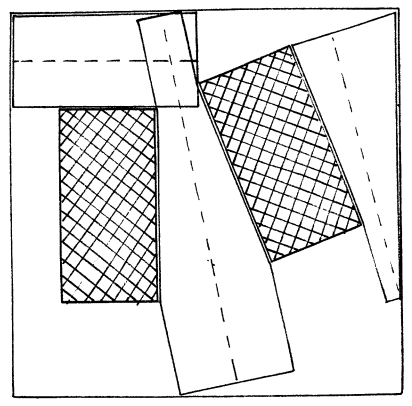
\includegraphics[width=0.35\textwidth]{images/cones.png}
        \caption{Muestreo del escenario por parte de ambos métodos}
        \label{fig:muestreo_metodos}
\end{figure}  

La mayor diferencia se encuentra en el modo de muestrear el espacio. El Q-PRM soluciona esto creando una secuencia determinista de muestras pseudo-aleatorias que conformarán un grafo a través del cual se buscará el camino mas rápido, mientras que en el caso del método de los conos generalizados se busca representar el espacio libre empleando dicha figura geométrica para luego buscar el camino. En la figura \ref{fig:muestreo_metodos} se puede observar como trabajan ambos métodos\\

Esta es una de las desventajas del algoritmo planteado por Brooks, ya que necesita representar todo el $C_free$ para encontrar una trayectoria, mientras que en el Q-PRM solo necesitas saber que los nodos y las conexiones que conforman el grafo no colisionan con ningún obstáculo. Además de esto, la complejidad de implementar el Q-PRM es bastante inferior, ya que utiliza conjuntos de muestras ya definidos en el campo de las matemáticas, por lo que todo se reduce a elegir cual de los distintos grupos se va a utilizar. En cuanto a la crítica que Yongji Wang hace al trabajo de Brooks, igualmente sería aplicable al algoritmo Q-PRM, ya que también sería necesario poder realizar movimientos de rotación pura.
\chapter{Caso de uso}
\label{caso_de_uso}

En este capítulo presentaremos el problema elegido como caso de uso para nuestra implementación, así como la justificación de por qué se ha elegido este problema y por qué es adecuado para el algoritmo implementado. Por último se hablarán de las limitaciones y el ámbito de uso del algoritmo.\\


\section{Descripción del problema}
\label{problema}

El programa realizado se basa en una aplicación típica de robots rastreadores de competición. En estas competiciones, los robots pasan por diferentes pruebas, como encontrar la salida de un laberinto o cruzar un escenario con obtáculos. En la figura \ref{fig:competi1}, puede observarse cómo estos obstáculos generalmente no tienen texturas y utilizan formas muy básicas. Con esto se intenta abstraer al robot de perturbaciones físicas y visuales, presentando un entorno modular y simple.

\begin{figure}[h]
		\centering
        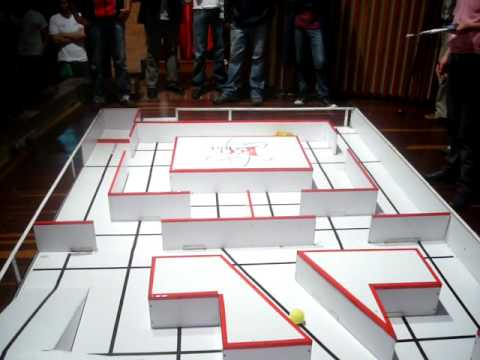
\includegraphics[width=0.5\textwidth]{images/competi1.jpg}
        \caption{Escenario de competición robótica}
        \label{fig:competi1}
\end{figure}  

El uso de obstáculos modulares permite simular una gran cantidad de casos problemáticos, siendo muy fácil reconfigurar su posición y unir obstáculos para crear obstáculos más complejos.

En el programa desarrollado, el robot pasará un total de tres pruebas diferentes en las que se combinarán distintos obstáculos frecuentes en las competiciones de robots rastreadores. Además, se tendrá en cuenta el tiempo usado en recorrer el escenario, por lo que se intentará minimizar.



\section{Justificación del algoritmo}
\label{justificacion}

\comment{??}



\section{Ámbito de uso}
\label{ambito}

\comment{?? limitaciones??}
\chapter{Implementación}
\label{implementacion}

En este capítulo se detalla la implementación tanto del algoritmo seleccionado como el desarrollo de la simulación. Se mostrarán los aspectos referentes del modelado del entorno así como el diseño del controlador del robot. Además, se muestra la composición del algoritmo y su desarrollo.

\section{Simulación}
\label{simulacion}

Para testar el funcionamiento del algoritmo se han realizado diferentes experimentos sobre el entorno de simulación robótica V-REP. V-REP es un simulador muy versátil que permite diferentes opciones a la hora de integrarse en un proyecto. Por un lado, está basado en el lenguaje Lua y ofrece un interprete integrado en el propio simulador, sin embargo, también permite utilizar programas externos en diversos lenguajes de programación como son: C++, Python o Java. Además, V-REP está integrado en ROS y pone a disposición del usuario los paquetes necesarios para realizar simulaciones de proyectos basados en ROS. En el caso que nos ocupa, se ha utilizado el lenguaje Python a través de la API proporcionada por V-REP para el control remoto de la simulación.

\subsection{Robot seleccionado}

Como base para implementar los algoritmos, se ha seleccionado un robot móvil con dos grados de libertad y configuración holonómica. V-REP contiene varios modelos de robots reales de este tipo, tales como: el Khepera , E-Puck o el Pioneer 3D-X. Se ha utilizado este último, mostrado en la figura \ref{fig:pioneer}, dado que es un robot bastante usado en tareas de navegación, y su relación entre tamaño y prestaciones es adecuada para nuestro problema.

\begin{figure}[h]
		\centering
        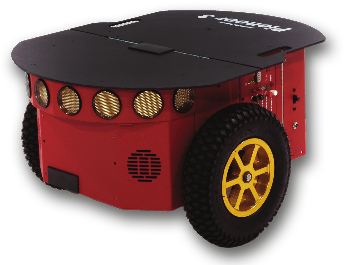
\includegraphics[width=0.5\textwidth]{images/pioneer.png}
        \caption{Robot Pioneer 3D-X}
        \label{fig:pioneer}
\end{figure} 

El Pionner 3D-X es un robot móvil impulsado por dos ruedas de movimiento diferencial. Junto a sus motores equipa encoders incrementales de 500 posiciones. También incluye sensores ultrasonicos de posición. Sin embargo, en esta aplicación no ha sido necesario utilizar ningún sensor interno del robot. El Pionner 3D-X tiene unas dimensiones de 38.1x45.5x23.7 cm. Su velocidad se acerca a los 1.6 m/s y tiene una capacidad de carga de hasta 23 kg.

\subsection{Desarrollo del controlador del robot}

La API remota de V-REP proporciona acceso al control de los actuadores del robot. Tomando como base la modificacion de parámetros de bajo nivel de los actuadores (velocidad y sentido de giro), se ha desarrollado un controlador que permite al robot desplazarse entre dos puntos con un error menor a 10cm. Teniendo en cuenta el tamaño del robot, se considera que es una precisión muy razonable.\\

El primer controlador implementado ha sido la función de giro y orientación. En nuestra aplicación, es muy importante realizar giros controlados, ya que repercutirán con gran importancia en la suavidad de los movientos del robot, así como en el tiempo ocupado en realizar la prueba. Por una parte, se requiere conocer en todo momento la orientación del robot respecto al eje de coordenadas global del simulador. Al mismo tiempo, el controlador debe permitir modificar esta orientación con el objetivo de dirigir el robot correctamente hacia los puntos objetivos. A continuación, en la figura \ref{fig:flujogiro} se muestra un diagrama de estados en el que se define el modo de actuación del robot tras una orden de giro.\\

\begin{figure}[H]
		\centering
        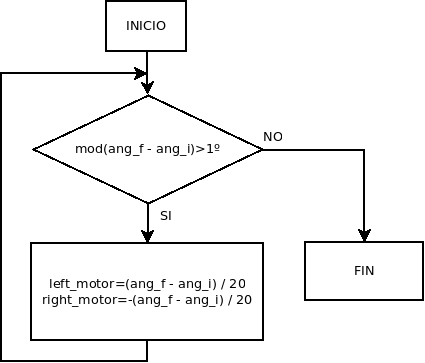
\includegraphics[width=0.5\textwidth]{images/flujogiro.png}
        \caption{Diagrama de estados del controlador de giros}
        \label{fig:flujogiro}
\end{figure} 

El segundo controlador del robot corresponde a su traslación. Ya que el robot constituye el punto de inicio de cualquier trayectoria que sea desarrollada, se debe conocer su posición inicial antes de correr el algoritmo de planificación. También, durante la simulación, se requiere un conocimiento en tiempo real de la posición global del robot. Este controlador nos permitirá definir el desplazamien y la consecución de objetivos del robot. En el siguiente diagrama de estados, representado en la figura \ref{fig:flujoavance}, se muestra la implementación de este controlador.

\begin{figure}[H]
		\centering
        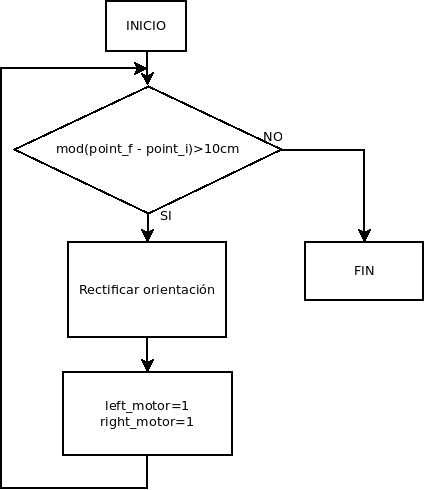
\includegraphics[width=0.5\textwidth]{images/flujoavance.png}
        \caption{Diagrama de estados del controlador de desplazamiento}
        \label{fig:flujoavance}
\end{figure} 

\subsection{Escenarios de simulación}

Los escenarios propuestos se han diseñado para probar la eficacia del algoritmo frente a diferentes situaciones problemáticas. Entre los puntos críticos de los escenarios destacan: tuneles con una altura definida, pasillos estrechos y zigzagueos. El uso de bloques sólidos modulares permite realizar configuraciones precisas para probar de forma directa las capacidades del algoritmo. Se han diseñado 3 escenarios con un area de 10x7.5m.

\begin{itemize}
	\item Escenario A: Túneles y obstáculos de diferente altura. Puede observarse en la figura \ref{fig:escenario1}.	
	
	
\begin{figure}[H]
		\centering
        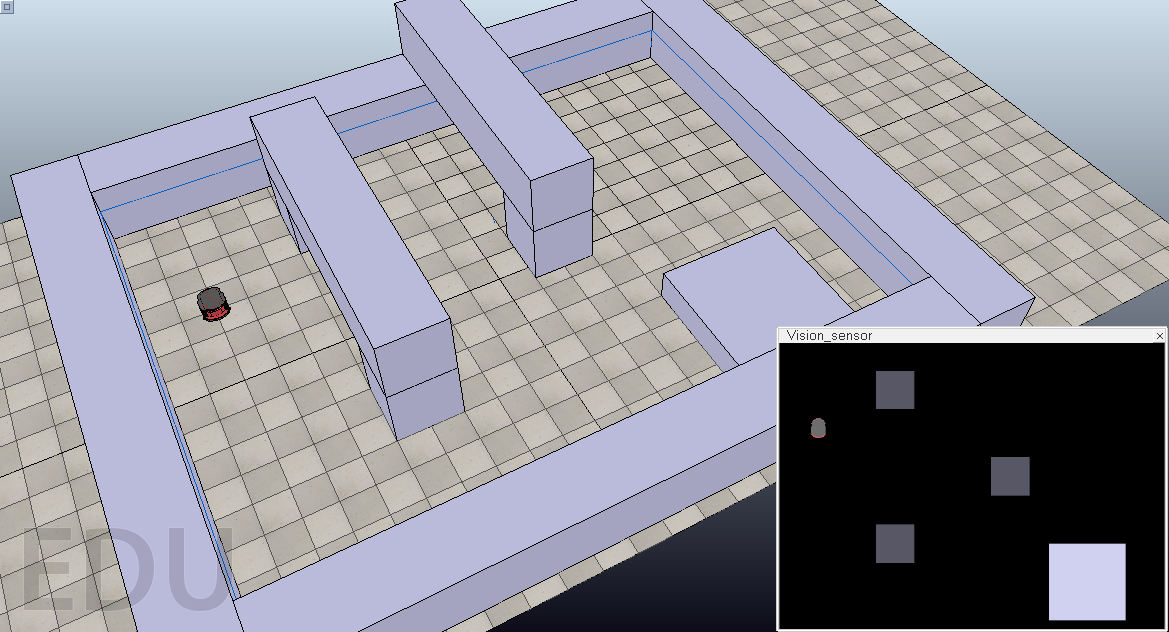
\includegraphics[width=0.7\textwidth]{images/escenario1}
        \caption{Escenario número 1}
        \label{fig:escenario1}
\end{figure} 
	
	\item Escenario B: Zigzagueo constante y pasillos estrechos. Puede observarse en la figura \ref{fig:escenario2}.
	
		
\begin{figure}[H]
		\centering
        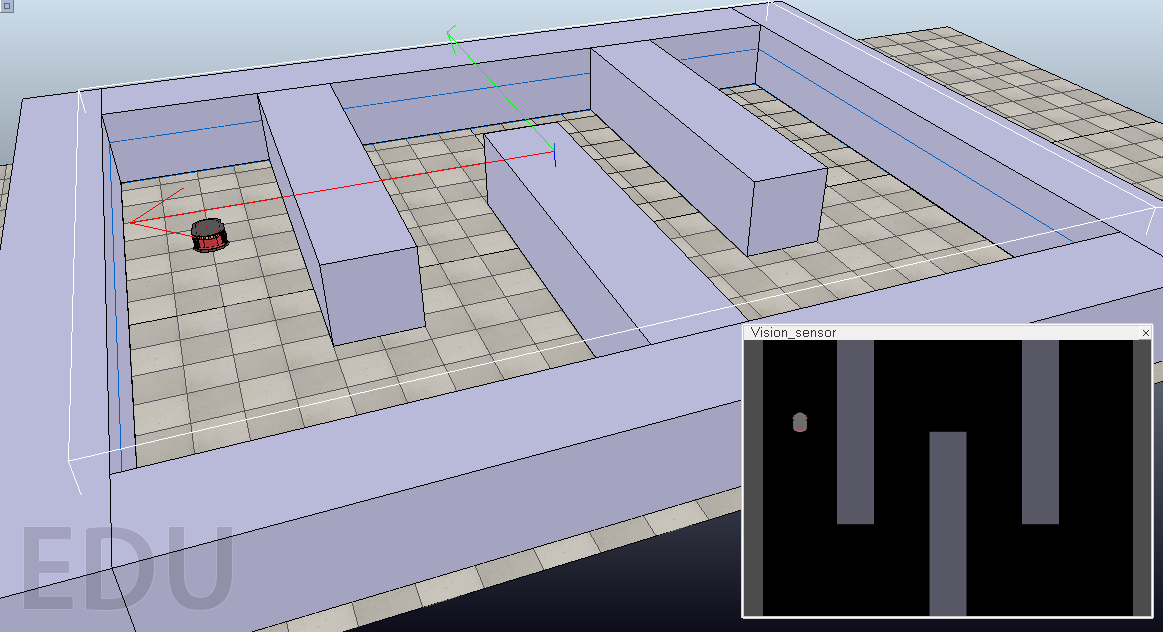
\includegraphics[width=0.7\textwidth]{images/escenario2.png}
        \caption{Escenario número 2}
        \label{fig:escenario2}
\end{figure} 
	
	\item Escenario C: Integración de túneles, zigzagueos y pasillos estrechos. Puede observarse en la figura \ref{fig:escenario3}.

	
\begin{figure}[H]
		\centering
        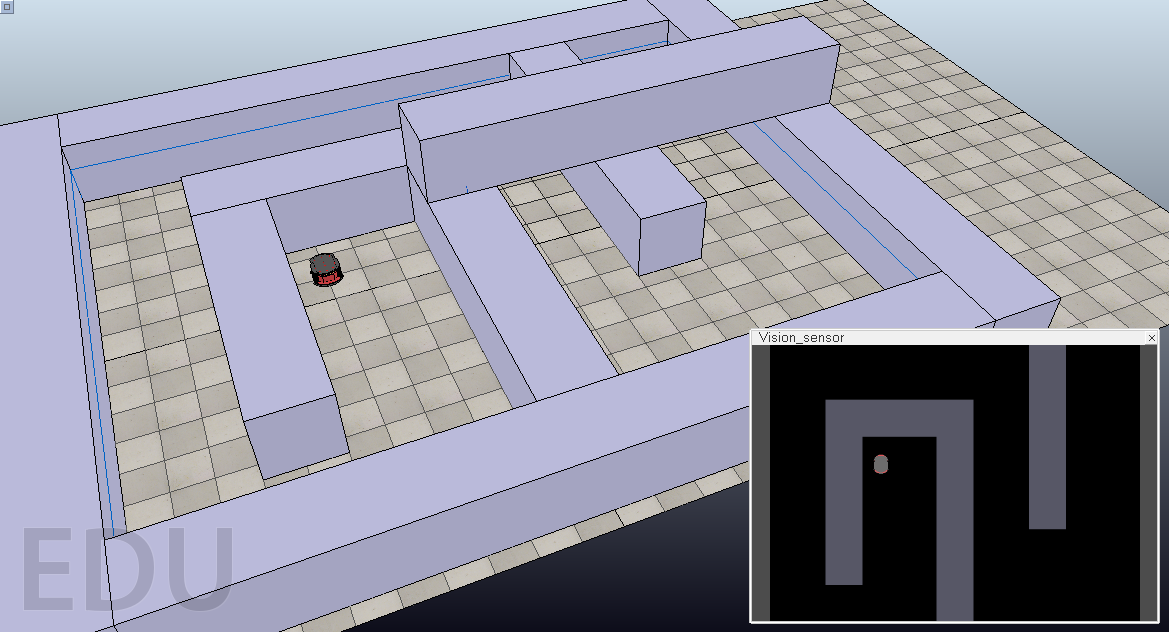
\includegraphics[width=0.7\textwidth]{images/escenario3.png}
        \caption{Escenario número 3}
        \label{fig:escenario3}
\end{figure} 

\end{itemize}




\subsection{Extracción de datos del simulador}

Uno de los puntos mas interesantes al trabajar con V-REP es la generación de planos a partir de los escenarios. La aplicación desarrollada está programada para funcionar en dos dimensiones, sin embargo, para crear los mapas se han tenido en cuenta tres dimensiones. El motivo de esto es obtener un funcionamiento óptimo del robot en situaciones cuya cruzabilidad se vea comprometida. Los casos más numerosos son aquellos en los que el robot se enfrenta al paso bajo un obstáculo elevado. 

Para extraer el plano se ha utilizado una cámara aérea de proyección ortogonal. Su rango de visión abarca la superficie completa del escenario y está situada a una altura ligeramente superior a la del robot. Dicho de otra forma, la cámara captará todos los objetos que se encuentren en el escenario que intercedan en el volumen mínimo sobre el que puede garantizarse la cruzabilidad.

En las imágenes de la figura \ref{fig:tunel} se puede observar que los obstáculos cuya altura es superior al robot, no se tienen en cuenta a la hora de procesar el algoritmo.

	
\begin{figure}[h]
		\centering
        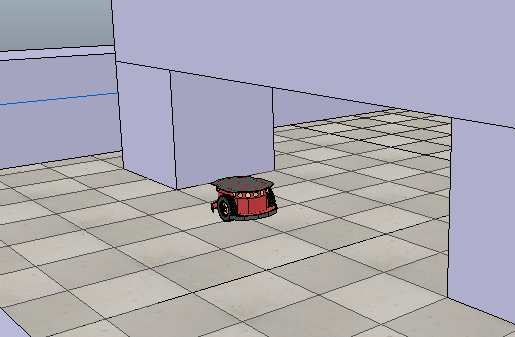
\includegraphics[width=0.7\textwidth]{images/tunel.png}
        \caption{Obstáculo elevado. La linea azul del fondo representa la altura mínima requerida para garantizar la cruzabilidad.}
        \label{fig:tunel}
\end{figure} 

Las imágenes son transferidas desde el simulador al programa principal, dónde se les aplica el algoritmo y comienza la ejecución.


\section{Algoritmo}
\label{algoritmo}

En esta sección se presenta el algoritmo que se ha implementado para el caso de uso que se ha tratado. El algoritmo se puede ver en el flujograma de la figura \ref{fig:flujo_algoritmo}. \\

\begin{figure}[H]
		\centering
        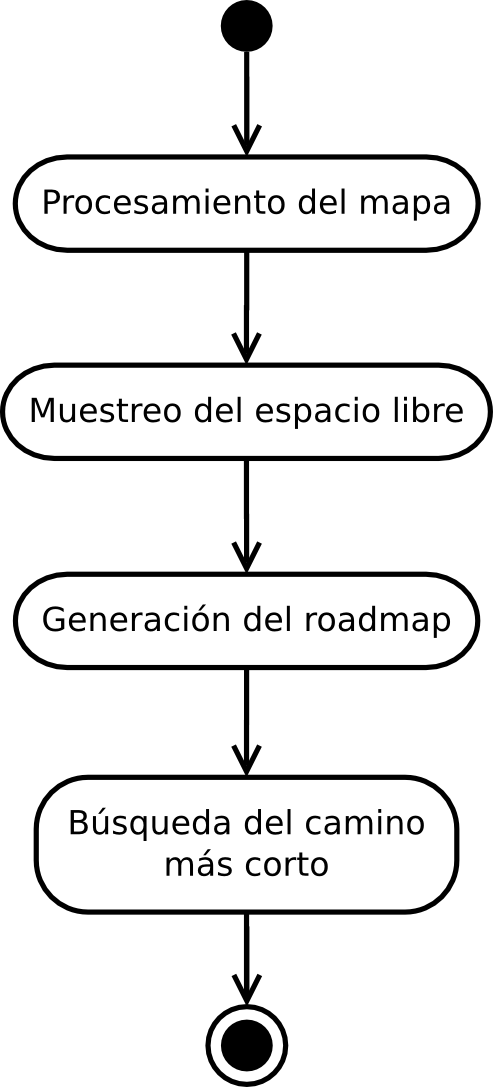
\includegraphics[width=0.2\textwidth]{images/flujo_main.png}
        \caption{Flujograma principal del algoritmo completo}
        \label{fig:flujo_algoritmo}
\end{figure} 


En primer lugar se procesa la imagen obtenida del escenario (mapa) para extraer los obstáculos. A continuación, se generan los puntos (muestras) que corresponderán a los nodos del roadmap y se conectan siguendo un criterio de distancias. Por último, cuando un punto inicial y un punto final son pedidos, se incluyen en el grafo y se calcula el camino más corto mediante un algoritmo de búsqueda en grafos, tal como el Djisktra o el $A^*$.\\

\subsection{Procesamiento del mapa}

A partir de la imagen del escenario capturada desde el simulador, se realiza un procesamiento de la misma usando técnicas de visión por computador. Se comienza por realizar un umbralizado de manera que el resultado es una imagen binaria en la que los obstáculos son píxeles blancos y el espacio libre píxeles negros. \\

A la imagen binaria se le realiza un etiquetado de objetos para obtener los contornos de los distintos obstáculos, los cuales son posteriormente simplificados para reducir el número de puntos que definen el obstáculo, mejorando la eficiencia del algoritmo de detección de colisiones.\\

Estos contornos que definen a los obstáculos son usados en posteriores partes del algoritmo. En la figura \ref{fig:procesado_imagen} se especifica el diagrama de flujo del procesamiento del mapa.\\

\begin{figure}[H]
		\centering
        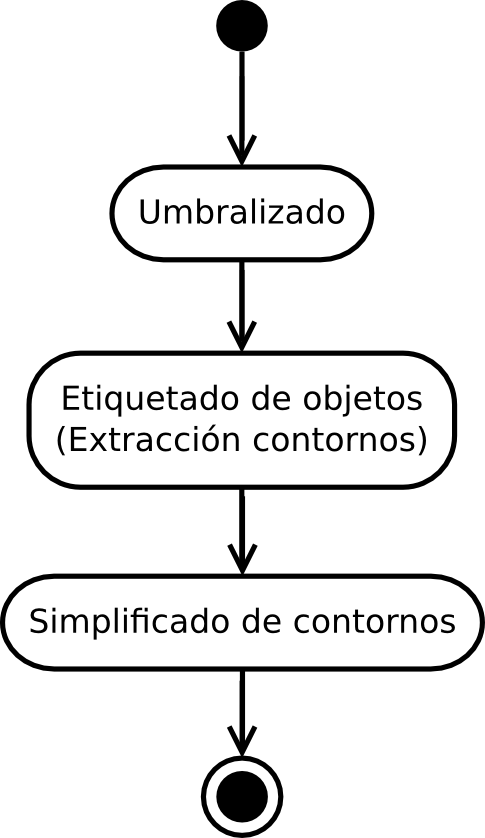
\includegraphics[width=0.2\textwidth]{images/flujo_imagen.png}
        \caption{Flujograma principal del procesamiento del mapa}
        \label{fig:procesado_imagen}
\end{figure} 

\subsection{Muestreo del espacio libre}

El siguiente paso para la generación del roadmap es el muestreo del espacio libre. En el algoritmo original este muestreo se realiza de forma aleatoria, generando nodos del roadmap repartidos aleatoriamente por todo el entorno. La mejora que introduce el artículo que es objeto de estudio con este caso práctico es la generación de dicho muestreo a partir de conjuntos de puntos cuasi-aleatorios. Estas distribuciones de puntos tienen la ventaja de ocupar el espacio libre de forma más eficiente, por lo que con menos cantidad de puntos se puede abarcar un área mayor y, por tanto, más partes delicadas del mapa. Estas partes delicadas pueden ser, por ejemplo, estrechamientos del espacio libre entre obstáculos. Los autores del artículo dan una medida de la ocupación eficiente del espacio libre con un parámetro que ellos llaman \textit{discrepancia}:\\


 \[ D_N(P) = \sup_{j}{\left| \frac{A(J)}{N} -  \mu(J) \right| }\]\\

En la que P es un conjunto de N puntos d-dimensionales, $\left\lbrace x_0, ... , x_{N-1} \right\rbrace$ en $[0,1]^d$, J es cualquier subconjunto rectangular de $[0,1]^d$, $\mu(J)$ es su medida n-dimensional y A(J) es el número de puntos contenido en $P \cap J$.\\

Para el muestreo de puntos cuasi-aleatorios se han usado dos distribuciones de puntos: el conjunto de Hammersley y el conjunto de Halton. Estas distribuciones se generan a partir de una semilla para un número arbitrario de dimensiones. Estas distribuciones se pueden calcular de la siguiente manera:

\subsubsection{Conjunto de Hammersley}

Dados $d-1$ números primos distintos $p_1, p_2, ... , p_{d-1}$ el i-ésimo punto del conjunto es dado por la expresión:

\[ \left( \frac{i}{N}, r_{p_1}(i), ..., r_{p_{d-1}(i)} \right), \qquad i = 0, 1, ..., N-1\]

\subsubsection{Conjunto de Halton}

Dados $d$ números primos distintos $p_1, p_2, ..., p_d$ el i-ésimo punto del conjunto es dado por la siguiente expresión:

\[ \left( r_{p_1}(i),  r_{p_2}(i), ...,  r_{p_d}(i) \right) \]\\~\\

%\subsubsection{Función $r_p(i)$}
En ambos casos, la función $r_p(i)$ se obtiene  escribiendo los dígitos de la notación basada en $p$ en orden inverso. Por ejemplo, para la expresión $i = a_0 + a_1 p + a_2 p^2 + a_3 p^3 + ... $ donde $a_j \in \left\lbrace 0, 1, ... , p-1 \right\rbrace$ la función $r_p(i)$ sería:\\

\[ r_p(i) = \frac{a_0}{p} + \frac{a_1}{p^2} + \frac{a_2}{p^3} + \frac{a_3}{p^4} + ...\]\\

\comment{pasarlo a impersonal}\\

Para nuestra implementación se ha usado una biblioteca ya existente, perteneciente al paquete cgkit que proporciona estos conjuntos de puntos de manera cómoda y rápida, ahorrando tiempo de desarrollo y depuración de errores. La figura \ref{fig:muestreo} muestra una comparativa de los distintos métodos de generación de puntos de muestreo en un escenario ficticio.\\

\begin{figure}[b]
		\centering
        \begin{subfigure}[b]{0.3\textwidth}
                \centering
                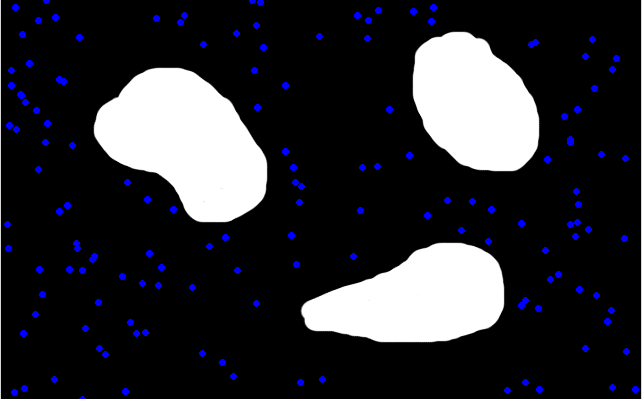
\includegraphics[width=\textwidth]{images/random.png}
                \caption{Muestreo aleatorio}
                \label{fig:muestreo_aleatorio}
        \end{subfigure}
        ~
        \begin{subfigure}[b]{0.3\textwidth}
                \centering
                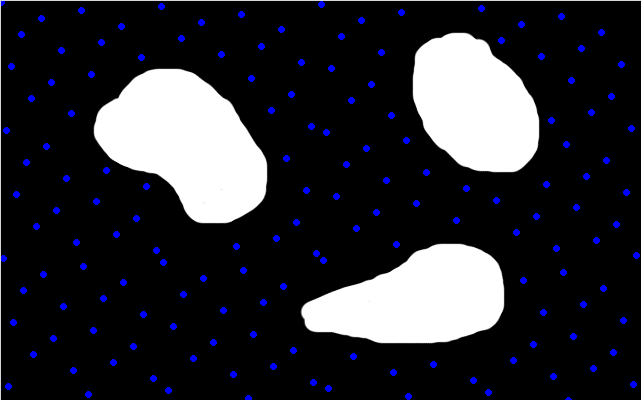
\includegraphics[width=\textwidth]{images/hammersley.png}
                \caption{Muestreo con puntos Hammersley}
                \label{fig:muestreo_hammersley}
        \end{subfigure}
        ~
        \begin{subfigure}[b]{0.3\textwidth}
         	   \centering
                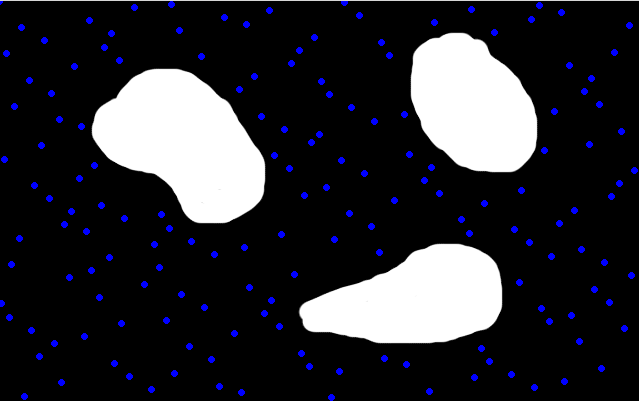
\includegraphics[width=\textwidth]{images/halton.png}
                \caption{Muestreo con puntos Halton}
                \label{fig:muestreo_halton}
        \end{subfigure}
        \caption{Comparativa de los distintos modos de muestreo del espacio libre}\label{fig:muestreo}
\end{figure}

\subsection{Creación del roadmap}
Una vez generados los puntos para el muestreo del espacio libre, se comprueba cada uno de los puntos comprobando colisiones con los obstáculos. Hemos desarrollado tres métodos distintos de comprobación de colisiones para este trabajo:

\begin{itemize}
\item \textbf{Detector de colisiones simple: } Este detector comprueba si el punto se encuentra dentro de alguno de los contornos que definen los obstáculos.
\item \textbf{Detector de colisiones con modelo del robot: } Este detector modela el robot como una circunferencia, y comprueba la colisión entre esta circunferencia y los contornos que definen los obstáculos-
\item \textbf{Detector de colisiones basado en convolución: } Al ser el detector anterior bastante lento en tiempo de cómputo, se aplica primero la convolución del círculo que representa al robot sobre toda la imagen, de forma que los obstáculos se dilatan. De esta forma se puede usar la detección de colisión simple, mucho más rápida, sobre los obstáculos dilatados, combinando las ventajas de los dos enfoques anteriores.
\end{itemize}

Tras eliminar los nodos que colisionan con obstáculos, se prodece a la conexión de los distintos nodos para la generación del grafo del roadmap. El criterio seguido para conectar dos nodos ha sido su vecindad. Se consideran vecinos dos nodos que estén a una distancia entre ellos menor que un valor umbral. Para cada pareja de nodos se calcula la distancia y se coloca en una matriz que reprensenta la conectividad del grafo, y que es usada como entrada de un algoritmo de búsqueda en grafos como Djisktra o $A^*$. Al ser la distancia del nodo A al nodo B la misma que la del nodo B al nodo A, sólo se calculan las distancias una vez.\\

Por último, y antes de añadir cada conexión al roadmap, se comprueba si esa arista del grafo es una trayectoria válida para el robot o colisiona con algún obstáculo, y sólo se añade en caso de que sea válida. Para la comprobación de la arista, se discretiza en diversos puntos, y se comprueba cada uno de ellos con alguno de los métodos presentados anteriormente.\\

\subsection{Busqueda del camino más corto}

Una vez se ha muestreado el espacio libre y se han conectado los nodos entre si para generar un grafo, el siguiente paso es buscar el camino más corto. Para ello se ha decidido implementar dos algoritmos diferentes, el $A^*$ y el Dijkstra. De esta forma se puede realizar un estudio acerca de como afecta a los resultados obtenidos el método que se elija para encontrar la trayectoria óptima.\\

\subsubsection{Algoritmo $A^*$}

El algoritmo $A^*$ fue presentado por primera vez por P. Hart, N. Nilsson y B. Raphael, miembros del Stanford Research Institute, en 1968, como una evolución del algoritmo de Dijkstra. Busca devolver la trayectoria que vaya del nodo inicial al final y que presente un coste más bajo. Mientras va explorando un camino mantiene otras posibles soluciones para cambiar de trayectoria, en caso de que la que se está recorriendo deje de ser óptima. Este algoritmo garantiza que siempre se encontrará una solución, si existe alguna.\\

El coste que se emplea para comparar las distintas posibles trayectorias entre sí viene dado por la suma de dos funciones. La primera es la distancia recorrida entre el nodo inicial y el nodo para el cual se está calculando el coste, mientras que la segunda consiste en una estimación de la distancia que es necesario recorrer para llegar al punto de destino. Aunque esto último se puede representar de diversas maneras, lo mas común es calcular la distancia en linea recta desde el nodo actual hasta el final.\\

A continuación se muestra el pseudocódigo que describe el algoritmo $A^*$ tal y como se ha implementado en este trabajo:\\

\begin{algorithm}
\caption{$A^*$ algorithm(start,target,distances,graph)}\label{A_algorithm}
\begin{algorithmic}[1]
\State openset = start
\State closedset = empty
\State path = empty
\State node connection = empty
\While {openset != empty and current != target}
	\For{nodes in graph}
 		\State Pick the current node neighbours
 		\If{neighbour not in openset and not in closedset} 
 			\State Calculate the cost value for that neighbour
 			\State Add that neighbour to openset
 			\State Add current,neighbour to node connection
 		\EndIf
	\EndFor
	\State current = best node in openset
	\State Add current to closedset and remove it from openset
	\EndWhile
		\If{exist path}
			\While{current != start}
				\State Add current to path
				\State current = node connection[current]
			\EndWhile
		\Else
			\State path = empty
		\EndIf
	\State return path
\end{algorithmic}
\end{algorithm}  

Al algoritmo se le pasan cuatro parámetros. Start hace referencia al nodo de origen, target es el nodo de destino, graph es un vector donde se almacenan los diversos puntos con los que se ha muestreado el $C_free$ y, por último, dist es una matriz donde se almacena la distancia de cada nodo a todos los demás. Si esos nodos son vecinos la distancia será la separación entre puntos y si no lo son, vale -1.\\

El $A^*$ trabaja con dos subconjuntos de nodos. En openset se almacenarán los ultimos nodos sobre los que se está trabajando (el nodo actual y el último nodo considerado de cada una de las trayectorias alternativas) mientras que en closedset se irán guardando los nodos por los que ya se haya pasado. Además, en node\_connection se almacena cada nodo del openset y el nodo contiguo en su trayectoria.\\

Se buscan los vecinos del nodo sobre el que se está trabajando, y, si no pertenecen ni a openset ni a closedset, se calcula su coste y se almacenan en openset. Una vez hecho esto, se elige al nodo de openset con menor coste y se pasa a trabajar sobre este. Este proceso se repite hasta que se llegue al nodo final o hasta que no queden nodos en openset.\\

Por último, si se ha encontrado un camino, se recorren los nodos almacenados en node\_connection y se reconstruye el camino. Si no se ha encontrado una trayectoria posible, se devuelve el path vacío y se dá un mensaje indicando el fallo.\\
\\

\subsubsection{Dijkstra}

Este algoritmo fue desarrollado originalmente por E. Dijkstra en 1956 como un método para encontrar el camino mas corto entre dos nodos, aunque existe otra versión, más utilizada, en la que se busca el camino más corto desde un nodo hasta todos los demás. Se puede optimizar el tiempo de ejecución utilizando una cola de prioridad (estructura de datos en las que a cada elemento se le asocia una prioridad que indica el orden en el que se van a devolver). En este algoritmo, el coste de cada nodo (tambien llamado prioridad) se calcula como la distancia entre este y el nodo inicial.\\ 

En este proyecto se ha recurrido a una implementación de la cola de prioridad desarrollada sobre el paquete de python heapq y publicada en un blog sobre python. Dicha implementación  proporciona cuatro funciones:\\

\begin{enumerate}
\item Constructor: Crea una cola de prioridad vacía o a partir de una estructura ya existente.
\item insert: Introduce un elemento en la cola de prioridad con su respectiva prioridad. También se puede usar para actualizar la prioridad de un elemento que ya está en la cola.
\item delete: Elimina un elemento de la cola de prioridad.
\item pop: Devuelve el elemento de la cola con la prioridad mas baja y lo quita de la cola. 
\end{enumerate}

A continuación se muestra el pseudocódigo del algoritmo:\\

\begin{algorithm}
\caption{Dijkstra algorithm(start,target,distances,graph)}\label{dikjstra}
\begin{algorithmic}
\State Create a priority queue pq
\State closedset = empty
\State path = empty
\State node connection = empty
\ForAll{nodes in graph}
 	\If{node == start}
 		\State Add node to pq with priority 0
 	\Else
 		\State Add node to pq with priority 10000
 	\EndIf
\EndFor
\While {pq != empty and current != target}
	\State Store in current the element with lower priority and add it to closedset
	\For{nodes in graph}
 		\State Pick the current node neighbours
 		\If{neighbour not in closedset} 
 			\State Calculate the cost value for that neighbour
 			\State Add that neighbour to pq or update its priority if it is already in
 			\State Add current,neighbour to node connection
		\EndIf
	\EndFor
\EndWhile
\If{exist path}
	\While{current != start}
		\State Add current to path
		\State current = node connection[current]
	\EndWhile
\Else
	\State path = empty
\EndIf
\State return path
\end{algorithmic}
\end{algorithm}

Se le pasan los mismos parámetros que al $A^*$. En este caso solo es necesario un conjunto de nodos, closedset, ya que la cola de prioridad hace la función de openset. Lo primero que se debe hacer es crear la cola y llenarla con todos los nodos del grafo. Al nodo inicial se le asignará una prioridad muy baja y al resto de nodos se les asignará una muy alta.\\

Una vez inicializada la cola de prioridad, se estrae el elemento con la prioridad mas baja, se buscan sus vecinos, se calcula su coste y se introducen en la cola de prioridad, donde la prioridad de cada nodo será su coste. Una vezs se ha hecho esto para todos los vecinos, se vuelve a extraer el nodo con la prioridad mas baja y se repite el proceso.\\

Al igual que antes, si se ha encontrado un camino se irá recorriendo el array node connections para formar la trayectoria, y si no, se devuelve el camino vacío junto con un mensaje indicando que no existe ninguna trayectoria.

\subsection{Simplificación de la trayectoria}

Una vez se extrae el camino más corto utilizando uno de los dos algoritmos implementados, se trata de simplificar la trayectoria final. Para esto, se coge el nodo inicial y otro nodo más, dejando un nodo entre medias. Se comprueba si es posible ir directamente de uno a otro sin chocar con ningun obstáculo y, en caso afirmativo, se elimina el nodo intermedio, al no ser necesario. Se coge el siguente nodo de la trayectoria y se intenta llegar desde el inicial y se repite el proceso hasta que se tenga un nodo al que no se puede llegar. Una vez hecho esto, se parte de dicho nodo y se intenta llegar al siguiente nodo, dejando uno entre medias y se vuelve a empezar con el proceso hasta que la trayectoria cuente con el número mínimo de nodos necesarios para llegar del punto inicial al final sin problema.\\

\section{Resultados}
\label{resultados}

\comment{Resultados y explicación de cómo afecta cada cosa al resultado}
\chapter{Conclusiones}
\label{Conclusiones}

\comment{Conclusiones y resultados y esas cosas}

%%%% Bibliography %%%%%%%%%%%%%%%%%%%%%%%%%%%%%%%%%%%%%%%%%%%%%%%%%%%%%%%%%%%%%
%\newpage
%\bibliographystyle{plain}
%\bibliography{Bibliography.bib}

\end{document}
